\begin{figure*}[htbp]
\centering
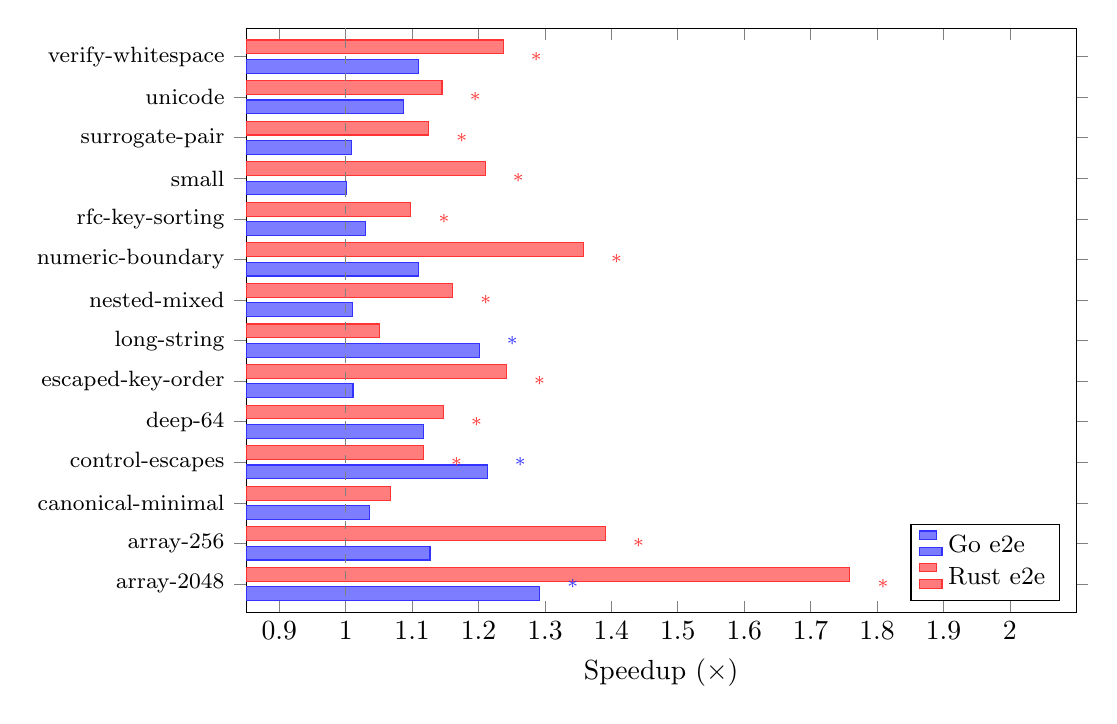
\begin{tikzpicture}
\begin{axis}[
    xbar,
    bar width=5pt,
    width=\textwidth,
    height=9cm,
    xlabel={Speedup ($\times$)},
    ytick={1,2,3,4,5,6,7,8,9,10,11,12,13,14},
    yticklabels={
        array-2048,
        array-256,
        canonical-minimal,
        control-escapes,
        deep-64,
        escaped-key-order,
        long-string,
        nested-mixed,
        numeric-boundary,
        rfc-key-sorting,
        small,
        surrogate-pair,
        unicode,
        verify-whitespace},
    y tick label style={font=\footnotesize},
    xmin=0.85,
    xmax=2.1,
    ymin=0.3, ymax=14.7,
    xtick={0.9, 1.0, 1.1, 1.2, 1.3, 1.4, 1.5, 1.6, 1.7, 1.8, 1.9, 2.0},
    legend style={at={(0.98,0.02)}, anchor=south east, font=\small},
    legend cell align={left},
    every axis plot/.append style={fill opacity=0.85},
    clip=false,
]
% Go CLI e2e canonicalize
\addplot[fill=blue!60, draw=blue!80] coordinates {
    (1.292, 1)
    (1.127, 2)
    (1.036, 3)
    (1.213, 4)
    (1.117, 5)
    (1.011, 6)
    (1.201, 7)
    (1.010, 8)
    (1.110, 9)
    (1.030, 10)
    (1.001, 11)
    (1.009, 12)
    (1.087, 13)
    (1.109, 14)
};
% Rust CLI e2e canonicalize
\addplot[fill=red!60, draw=red!80] coordinates {
    (1.759, 1)
    (1.391, 2)
    (1.067, 3)
    (1.117, 4)
    (1.147, 5)
    (1.242, 6)
    (1.051, 7)
    (1.161, 8)
    (1.358, 9)
    (1.098, 10)
    (1.210, 11)
    (1.125, 12)
    (1.145, 13)
    (1.237, 14)
};
\legend{Go e2e, Rust e2e}
% Reference line at 1.0x
\draw[dashed, gray, thin] (axis cs:1.0,0.3) -- (axis cs:1.0,14.7);
% BH-significant markers for Go (3 canonicalize: array-2048, control-escapes, long-string)
\node[font=\scriptsize, blue!80] at (axis cs:1.342, 1) {$*$};
\node[font=\scriptsize, blue!80] at (axis cs:1.263, 4) {$*$};
\node[font=\scriptsize, blue!80] at (axis cs:1.251, 7) {$*$};
% BH-significant markers for Rust (12 of 14 canonicalize)
\node[font=\scriptsize, red!80] at (axis cs:1.809, 1) {$*$};
\node[font=\scriptsize, red!80] at (axis cs:1.441, 2) {$*$};
\node[font=\scriptsize, red!80] at (axis cs:1.167, 4) {$*$};
\node[font=\scriptsize, red!80] at (axis cs:1.197, 5) {$*$};
\node[font=\scriptsize, red!80] at (axis cs:1.292, 6) {$*$};
\node[font=\scriptsize, red!80] at (axis cs:1.211, 8) {$*$};
\node[font=\scriptsize, red!80] at (axis cs:1.408, 9) {$*$};
\node[font=\scriptsize, red!80] at (axis cs:1.148, 10) {$*$};
\node[font=\scriptsize, red!80] at (axis cs:1.260, 11) {$*$};
\node[font=\scriptsize, red!80] at (axis cs:1.175, 12) {$*$};
\node[font=\scriptsize, red!80] at (axis cs:1.195, 13) {$*$};
\node[font=\scriptsize, red!80] at (axis cs:1.287, 14) {$*$};
\end{axis}
\end{tikzpicture}
\caption{CLI end-to-end speedup of \schubfach over \burgerdybvig by
workload (canonicalize mode, 15~repetitions each).  Asterisks ($*$) mark
BH-significant comparisons ($q < 0.05$).  The Rust within-language pair
achieves significance on 12 of 14~workloads; the Go pair on 3 of
14~workloads (canonicalize mode).  Process startup overhead
(${\approx}$1.3\,ms Go, ${\approx}$0.5\,ms Rust) attenuates the
algorithmic signal more strongly in Go.}
\label{fig:cli-significance}
\end{figure*}
